% This template was originally by R. Jacob Vogelstein
% Updated on March 1, 2010 by Noah J. Cowan
% Updated by Brian D. Weitzner, April 29, 2014
% Edited March, 2016 by Karla Hernandez
% Edited September, 2017 by Keisuke Sakaguchi

\documentclass[12pt,oneside,final]{thesis}
%\documentclass[12pt,oneside,draft]{thesis} %% for draft (single space)

\usepackage[english]{babel} % Multilingual support
\usepackage{blindtext} % blind text for testing like lipsum

%%%%%%%% ACL Style Bibliography %%%%%%%%%%
\usepackage[style=authoryear-comp,citestyle=authoryear,natbib=true,backend=bibtex,maxbibnames=99,sorting=nyt,isbn=false,doi=false,dashed=false,url=true]{biblatex}
\addbibresource{thesis.bib}
\newcommand{\newcite}[1]{\citet{#1}}
\renewcommand{\cite}[1]{\citep{#1}}
\newcommand{\longcite}[1]{(\citeauthor*{#1}, \citeyear{#1})}
\newcommand{\eg}[1]{\citep[e.g.,][]{#1}}
\newcommand{\ie}[1]{\citep[i.e.,][]{#1}}

%%%%%%%%%% Basic packages and settings %%%%%%%%%%
\usepackage[a-1b]{pdfx} % This is required from JHU library (https://www.library.jhu.edu/library-services/electronic-theses-dissertations/formatting-guidelines-checklist/)
\usepackage{amsmath,amsfonts}
\usepackage{amsthm}
\usepackage{graphicx}
\usepackage{array}
\usepackage{hyperref} 
\usepackage{setspace}
\usepackage{multirow}

\usepackage{enumitem}
\newlist{inlinelist}{enumerate*}{1}
\setlist*[inlinelist,1]{%
  label=(\arabic*),
}

\usepackage{fancyhdr}    % Use nice looking headers along with the required footer page numbers   

%Define the header/footer style
\pagestyle{fancy}
\fancyhf{}
\setlength{\headheight}{15pt}
\lhead{\leftmark}
\cfoot{\thepage}
\renewcommand{\headrulewidth}{0pt} % Remove line on page header by setting to 0pt
\fancypagestyle{plain}{% Redefine ``plain'' style for chapter boundaries
\fancyhf{} % clear all header and footer fields
\fancyfoot[C]{\thepage} % except the center
\renewcommand{\headrulewidth}{0pt}
\renewcommand{\footrulewidth}{0pt}}

%\makeglossary % enable the glossary

%%%%%%%%%%%%%%%%%%%%%%%%%%%%%%%%%%%%%%%%%%%%%%%%
% Personal customizations (e.g., macros)
% Personal macros are written here.
\usepackage{csquotes}

%%%%%%%%%%%%%%%%%%%%%%%%%%%%%%%%%%%%%%%%%%%%%%%%

\begin{document}

\title{\uppercase{JHU Minimum Dissertation Template for NLP}}
\author{Your Name Here}
\degreemonth{Month}
\degreeyear{Year} 
\dissertation
\doctorphilosophy
\copyrightnotice


% add your chapters, best way is to have separate TeX files for each chapter
%% FRONTMATTER
\begin{frontmatter}

% generate title
\maketitle

\begin{abstract}

\blindtext[3]

\end{abstract}

\begin{acknowledgment}

\blindtext[3]

\end{acknowledgment}

\begin{dedication}
 
\blindtext[3]

\end{dedication}

% generate table of contents
\tableofcontents

% generate list of tables
\listoftables

% generate list of figures
\listoffigures

\end{frontmatter}

\part{title for part I}
\chapter{Introduction}
\label{chap:intro}
\chaptermark{Optional running chapter heading}

This is a language game \cite{wittgenstein1953philosophical}.
By the way, \newcite{quine1951main} wrote ``Two dogmas of empiricism'',
\begin{displayquote}
  Modern empiricism has been conditioned in large part by two
  dogmas. One is a belief in some fundamental cleavage between
  truths which are analytic, or grounded in meanings independently of
  matters of fact, and truth which are synthetic, or grounded in fact.
  The other dogma is reductionism: the belief that each meaningful
  statement is equivalent to some logical construct upon terms which
  refer to immediate experience.
\end{displayquote}


A table is shown in Table \ref{tab:sample}.
\blindtext[3]

\begin{table}[t]
  \small
  \centering
  \begin{tabular}{l|c|c|c} \hline
       & A     & B & C \\ \hline\hline
  cat  & meow  &   &   \\
  dog  & woof  &   &   \\
  cow  & moo   &   &   \\ \hline
  \end{tabular}
  \caption{Sample table}
  \label{tab:sample}
  %\vspace{-2mm}
\end{table}

\blindtext[2]
A figure sample is shown in Figure \ref{fig:sample}.

\begin{figure}[t]
  \centering
  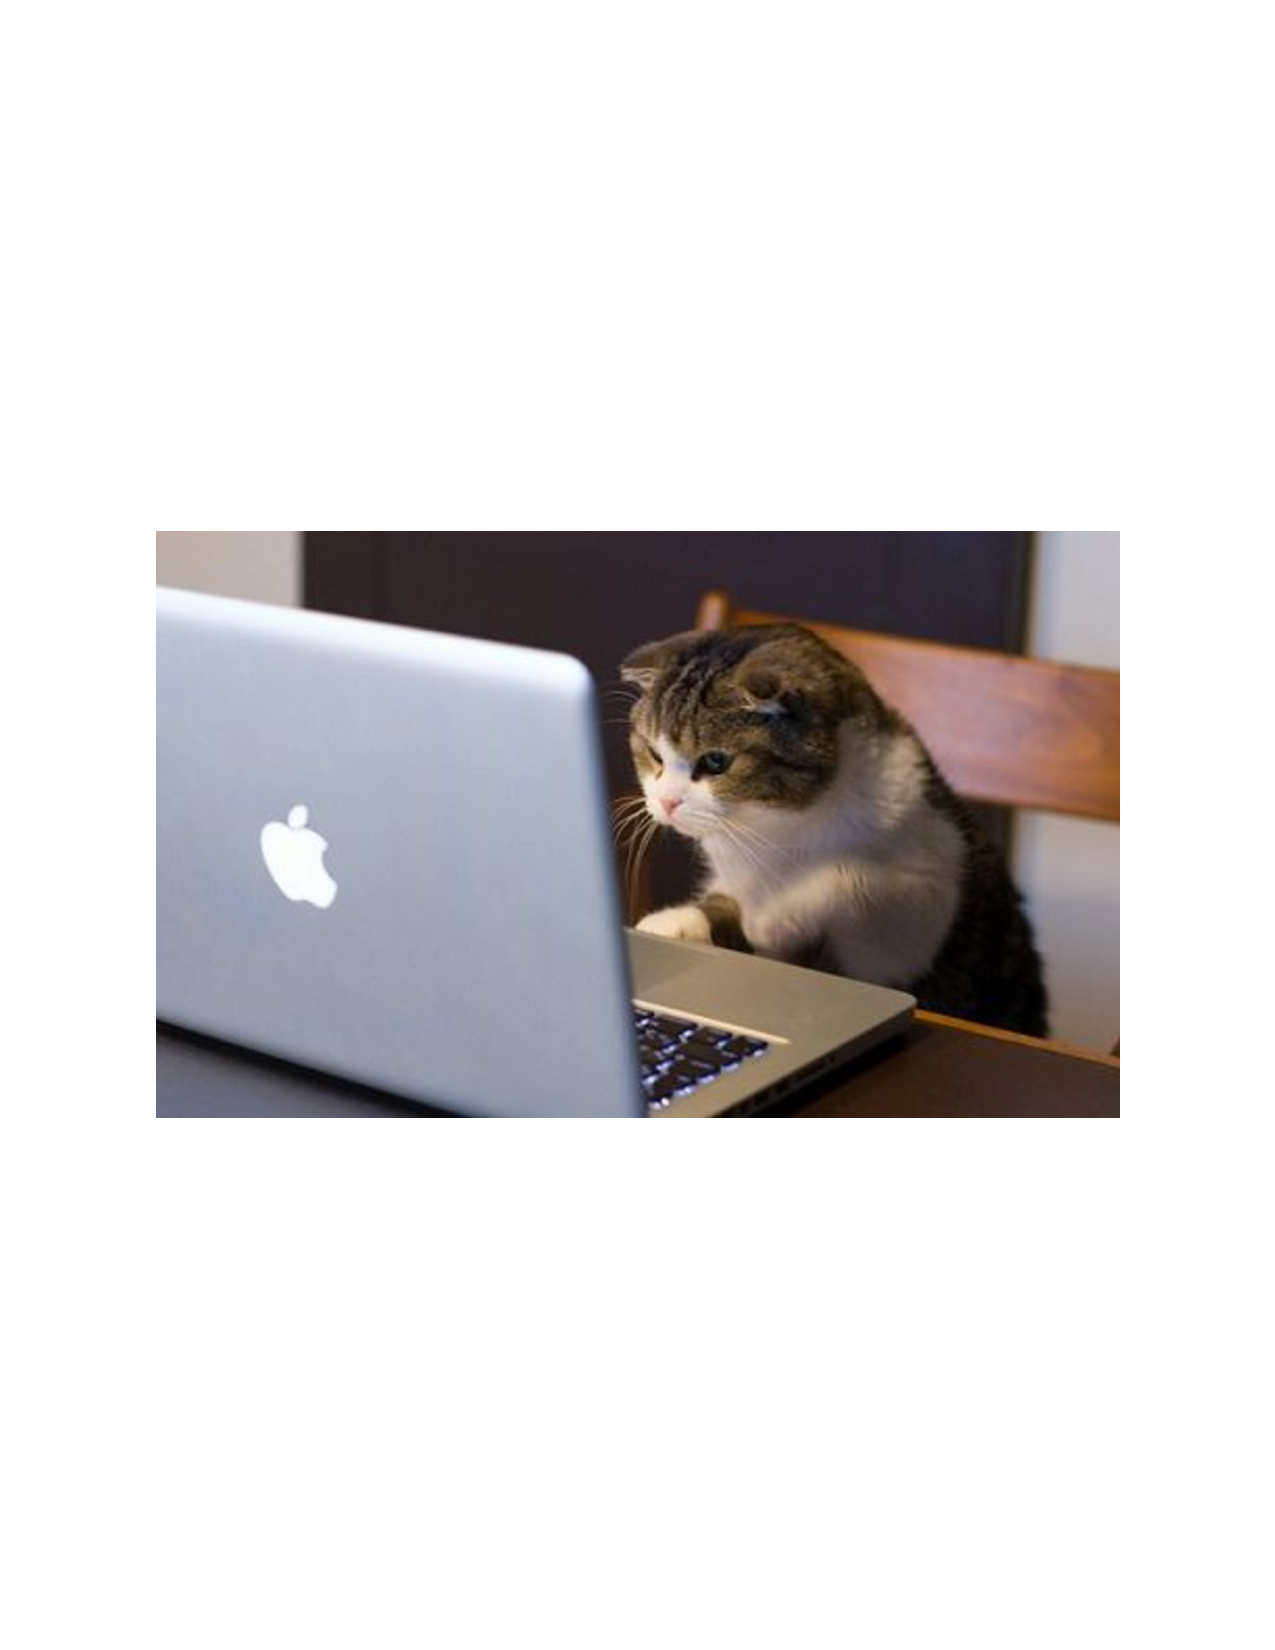
\includegraphics[width=70mm]{fig/sample_figure.pdf}
  \caption{Sample figure}
  \label{fig:sample}
  %\vspace{-2mm}
\end{figure}


\blindtext[3]


\part{title for part II}

\appendix
%!TEX root = root.tex
\chapter{Extra Stuff}
This is appendix.
\blindtext[2]


%% REFERENCES
% if you use BIBTEX

%\bibliographystyle{IEEEtran}
%\bibliography{IEEEabrv,thesis} % PLEASE USE THE APPROPRIATE BIBLIOGRAPHY STYLE FOR YOUR DISSERTATION !!!!!!!!!!!!!
\printbibliography

\begin{vita}

\Blindtext[1]

\end{vita}

\end{document}
